% --------------------------------------------------
% MG-Template for thesis, FEB 2020 v.1
% Das Dokument muss mit XeLaTeX kompiliert werden.
% --------------------------------------------------

% TODO: Bilder positionieren
% TODO: inhaltliches Probelesen

\documentclass[openright, twoside, utf8, 11.5pt]{scrbook}

% \usepackage[german]{babel}
% \usepackage[utf-8]{inputenc}
\usepackage{amsmath}
\usepackage{amssymb}
\usepackage{lipsum}
\usepackage{mgthesis}
\usepackage[binary-units=true]{siunitx}
\usepackage{tikz}

\sisetup{locale = DE}

\newcommand{\thesistype}{Projektarbeit}
\newcommand{\degreetype}{Bachelor/Master of Science (M./B.\,Sc.)}

\title{Qualitativer Vergleich von Beaterkennungsalgorithmen}
\author{Hannes Frank}
\date{19. Juli 2020}

\newcommand{\matnr}{4501110}
\newcommand{\gutachter}{Prof. Dr.-Ing. habil. Rainer Groh}
\newcommand{\betreuer}{M. Sc. Lars Engeln}


\begin{document}
	\color{mycolor}

	% Titelseite
	\makeatletter
\begin{titlepage}
	\RaggedRight
	
\includegraphics[width=0.35\textwidth]{resources/logoTUD.png}\par\vspace{0cm}
	\noindent\rule{\textwidth}{0.4pt}
	{\normalfont\mdseries\small\sffamily Fakultät Informatik,}
	{\normalfont\mdseries\small\sffamily Institut für Software- und Multimediatechnik, Professur für Mediengestaltung}
	\vspace{2mm}\noindent\hrule
	\vspace{3cm}
	{\normalfont\Large \thesistype \par}
	\vspace{1cm}
	{\normalfont\Huge\mdseries\sffamily \@title\par}
	\vspace{1.5cm}
	{\normalfont\large im Rahmen des Moduls:\par}
	{\normalfont\Large\bfseries INF-D-960 Analyse eines Forschungsthemas \par}
	\vspace{1cm}
	{\sffamily\large\mdseries erarbeitet von\par}
	\vspace{1.5mm}
	{\normalfont\Large \@author\par}
	\vspace{0.5mm}
	{\normalfont\large Matrikelnummer: \matnr \par}
	\vspace{2.0cm}
	{\sffamily\large Gutachter:\par}
    \vspace{1mm}
	{\normalfont\large \gutachter \par}
	\vspace{7mm}
	{\sffamily\large Betreuer:\par}
	\vspace{0.7mm}
	{\normalfont\large \betreuer \par}
	\vspace{1cm}
	{\sffamily\large\mdseries eingereicht am\par}
	\vspace{1mm}
	{\normalfont\normalsize \@date \par}
\end{titlepage}
\makeatother


	\cleardoublepage
	\begingroup
		\renewcommand*{\chapterpagestyle}{empty}
		\pagestyle{empty}
		\makeatletter
\chapter*{Selbstständigkeitserklärung}

\justifying Hiermit erkläre ich, dass ich die vorliegende Arbeit mit dem Titel \\

\vspace{0.5cm}
\centering
{\large\sffamily\mdseries \@title } \\
\vspace{1.0cm}
\justifying

selbstständig und ohne die Benutzung anderer als der angegebenen Hilfsmittel angefertigt habe. Alle Stellen, die wortwörtlich oder sinngemä\ss\ aus veröffentlichten oder nicht veröffentlichten Quellen entnommen sind, sind als solche kenntlich gemacht.\\

\vspace{2.5cm}
%\hfill \rule{0.33\textwidth}{0.4pt}\par
Dresden, \@date \hfill \@author
\makeatother
			\newpage
			\pagestyle{empty}
			\null\newpage
		\chapter*{Kurzfassung}

		\newpage
			\pagestyle{empty}
			\null\newpage
		\tableofcontents
		\cleardoublepage
	\endgroup

	% Inhalt
	% include = newpage; input = samepage
	\mainmatter
	\chapter{Einleitung}
\label{einleitung}
\acresetall

In diesem Kapitel wird die Zielsetzung dieser Arbeit
	und das Beaterkennungsproblem kurz erlkärt
	sowie dessen Anwendungsgebiete vorgestellt.

\section{Kontext}
{
	% leicht für Menschen, schwer für Maschinen
	Die Erkennung der regelmä{\ss}igen Schläge des Taktes eines Musikstücks ist eine triviale Aufgabe für Menschen.
	Manchmal tippen wir sogar unterbewusst unseren Fu{\ss} zum Takt der Musik,
		ohne aktiv darüber nachzudenken.
	Es ist jedoch sehr schwer diese Aufgabe zu automatisieren,
		da Maschinen kein Taktgefühl haben.
	Dennoch gibt es verschiedene Algorithmen,
		die genau das bewerkstelligen.
	% Anwendungen
	Diese Beaterkennungsalgorithmen werden z. B. in Videobearbeitungssoftware verwendet,
		um die visuelle Spur automatisch mit der Audiospur zu synchronisieren.
	Deshalb werden besonders beim Erstellen von Musikvideos solche Algorithmen eingesetzt.
	Auch in Audiobearbeitungs- und Aufnahmesoftware finden Beaterkennungsalgorithmen Einsatz,
		z. B. bei der automatischen Indizierung von Musikstücken.
	Bei Liveauftritten spielen Beaterkennungsalgorithmen auch eine wichtige Rolle.
	Hier werden sie eingesetzt um z. B. die Bühnenbeleuchtung automatisch und passend zur Musik zu steuern.
}

\section{Zielsetzung}
{
	Ziel dieser Arbeit ist es,
		einen umfangreichen, qualitativen Vergleich von ausgewählten Beaterkennungsalgorithmen zu erstellen,
		der hilfreich für die Auswahl eines geeigneten Algorithmus für einen Anwendungsfall ist.
	Dazu wurden drei Algorithmen analysiert und implementiert
		und mehrere Vergleichstests erstellt.
	Die Tests lassen die Algorithmen auf mit Beatpositionen annotierten Musikstücken laufen,
		beobachten dabei deren Ausgabe
		und vergleichen sie mit den Annotationen der Lieder.
	Auf diese Art und Weise werden mehrere Metriken zur Bewertung der Algorithmen erstellt,
		anhand welcher die Algorithmen verglichen werden.
}

\section{Kapitelübersicht}
{
	In Kapitel~\ref{grundlagen} werden für diese Arbeit relevante musikalische Grundbegriffe vorgestellt
		und die Grundlagen der Beaterkennung beschrieben.
	In Kapitel~\ref{verwandte_arbeiten} werden alle Paper,
		die im Rahmen dieses Forschungsprojekts verwendet wurden,
		kurz vorgestellt.
	In Kapitel~\ref{analyse} wird die Auswahl der für den Vergleich verwendeten Algorithmen begründet
		und deren genaue Funktionsweise beschrieben.
	In Kapitel~\ref{konzept} werden die Ziele des Vergleichs definiert,
		sowie dessen Aufbau und Umsetzung aufgezeigt.
	In Kapitel~\ref{ergebnisse} werden die Ergebnisse aller Tests vorgestellt und interpretiert.
	Es werden zu jedem Test mögliche Erklärungen für dessen Ergebnis abgegeben.
	Dabei wird in jedem Abschnitt eine der vier Forschungsfragen aus Kapitel~\ref{konzept} adressiert.
	In Kapitel~\ref{zusammenfassung} werden das Ziel der Arbeit, die Umsetzung des Vergleichs und das Resultat der Tests kurz zusammengefasst.
	Abschlie{\ss}end werden Ziele für zukünftige Vergleiche von Beaterkennungsalgorithmen vorgestellt.
}


	\chapter{Grundlagen und Begriffe}
\label{grundlagen}
\acresetall

In diesem Kapitel werden für diese Arbeit relevante musikalische Grundbegriffe vorgestellt
	und die Grundlagen der Beaterkennung beschrieben.

\section{Musikalische Grundbegriffe}
{
	Um die in dieser Arbeit untersuchten Beaterkennungsalgorithmen zu verstehen,
		wird etwas musikalisches Grundwissen benötigt.
	In diesem Abschnitt werden deshalbt Grundbegriffe erklärt,
		die in der restlichen Arbeit verwendet werden.

	\subsection{Takt}
	{
		Fast jedes Musikstück ist zeitlich in kurze und gleichlange Abschnitte unterteilt.
		Diese Abschnitte nennt man Takte
			und sie geben der Musik eine gewisse Struktur,
			da sich oft bestimmte Muster, wie z. B. Schlagzeugrhythmen, in jedem oder jedem zweiten Takt wiederholen
			und auch die Grenzen von Strophe, Refrain usw. an Taktgrenzen orientiert sind.
		Die Länge eines Taktes hängt von der Taktart und dem Tempo des Stücks ab
			und ist meist im einstelligen Sekundenbereich.
	}

	\subsection{Schlag (Beat)}
	{
		Ein Schlag (engl. Beat) ist eine Unterteilung des Taktes.
		Jeder Takt hat genau gleichviele Schläge (au{\ss}er es gibt einen Taktartwechsel im Stück).
		Die Abfolge von Schlägen in einem Lied ist oft dieselbe,
			die ein Mensch beim Hören der Musik intuitiv mit dem Fu{\ss} mitklopfen würde.
	}

	\subsection{Taktart}
	{
		Die Taktart besteht aus zwei Teilen
			und wird deshalb oft als ungekürzter Bruch angegeben (z. B. 4/4).
		Der Zähler gibt an,
			aus wie vielen Schlägen ein Takt besteht.
		Der Nenner gibt an,
			wie lange ein Schlag dauert
			und wird nicht in einer Zeiteinheit,
			sondern als Notenwert angegeben.
		Ein Nenner von 4 bedeutet z. B.,
			dass ein Schlag so lange wie eine Viertelnote dauert.
		Das ist für die musikalische Notation relevant,
			hat aber keine Bedeutung für diese Arbeit,
			da dahinter kein Bezug zur tatsächlichen Dauer (in Sekunden) eines Schlages steckt.
		Die meisten Lieder haben einen 4/4-Takt,
			weshalb manche Algorithmen in dieser Arbeit speziell auf diese Taktart ausgelegt sind.
	}

	\subsection{Tempo}
	{
		Das Tempo eines Musikstücks gibt an,
			wie schnell dieses gespielt wird.
		Es bestimmt somit die tatsächliche Dauer (in Sekunden) eines Schlages
			und wird in \ac{BPM} angegeben.
		Üblicherweise befinden sich Tempi von Musikstücken in einem Bereich zwischen 60 und 180 \ac{BPM}.
	}
}

\section{Grundlagen der Beaterkennung}
{
	Beaterkennung ist die Aufgabe,
		aus rohen Audiodaten die Anfangszeitpunkte der einzelnen Schläge eines Musikstücks zu extrahieren.
	Zusätzlich wird von manchen Algorithmen auch das Tempo berechnet.

	\paragraph{}
	{
		Das Beaterkennungsproblem bringt folgende Herausforderungen mit sich:
	}

	\paragraph{1} % kein eindeutiges Beatgeräusch
	{
		Es gibt nicht immer ein bestimmtes Geräusch,
			dass die Anfangszeitpunkte der Schläge markiert.
		Es kann sogar sein, dass auf einen Beat kein Signal kommt.
	}

	\paragraph{2} % Onsetungenauigkeit
	{
		Da oft viele Instrumente, mit sehr unterschiedlichen Klängen, in einem Lied spielen,
			ist es schwierig,
			besonders genaue Einsatzzeitpunkte von Noten zu bestimmen.
	}

	\paragraph{3} % Echtzeit
	{
		Bei der Beaterkennung in Echtzeit können nur Samples aus der Vergangenheit genutzt werden,
			wohingegen bei nicht-Echtzeit-Algorithmen alle Samples verwendet werden können.
	}

	\paragraph{4} % nicht trivial
	{
		Es ist keine effektive Methode die Lautstärkemaxima eines Audiosignals zur Beaterkennung zu nutzen,
			da es auch viele Peaks gibt,
			die nicht auf einen Beat passen.
	}

	\paragraph{5}  % Nichteindeutigkeit
	{
		Die Zuordnung von Audiodaten zu Beatzeitpunkten und Tempo ist nicht eindeutig.
		Schläge und Takte sind lediglich eine gedankliche Einteilung des Stücks,
			die man nicht direkt hören kann,
			sondern sich nur dadurch bemerkbar machen,
			dass musikalische Ereignisse
			(z. B. Anfang und Ende einer Note, Schlagzeugtöne oder Harmoniewechsel)
			an deren Grenzen orientiert sind.
		Man könnte also z. B. ein Stück mit 160 \ac{BPM} auch als eines mit 80 \ac{BPM} betrachten
			(angenommen der Zähler der Taktart ist durch zwei teilbar),
			indem man jeweils zwei Takte als einen interpretiert.
		Das Audiosignal wäre bei beiden Varianten das gleiche.
	}
}

	\chapter{Verwandte Arbeiten}
\label{verwandte_arbeiten}

\section{Zusammenfassung}


	\chapter{Analyse der Algorithmen}
\label{analyse}

\section{Selektion}
{
}

\section{Vergleich}
{
}

\section{Funktionsweise}
{
	% TODO: sagen, dass ich hier meine eigenen Implementierung beschreibe, welche aber dem Paper entsprechen sollte und wenn nicht schreib ichs dazu
	% TODO: vielleicht ein Wort zur Notation verlieren wegen Subscript und Klammern
	% * Subsxript t ist meistens Zeitreihenindex
	% * Subscripte sind meistens Indices für Zeitreihen, Arrays oder Matrizen
	% * manchmal werden Subscripte auch benutzt um verschiedene Versionen einer Variable zu differenzieren
	%   z. B. tau_f und tau_neu --> dann wern sa aber als Wörter geschrieben mit ner Text-Schriftart
	% * Zahlen in Klammern sind Parameter einer Funktion, die iwas mit diesen Zahlen macht
	% TODO: irgendwo erklären was ne ODF ist

	% Man könnte, wenn man noch Wörter braucht, noch viel mehr auf Implementierungsdetails eingehen, wie bestimmte Sachen umgesetzt wurden

	In diesem Abschnitt wird die Funktionsweise der verwendeten Algorithmen im Detail erklärt.
	Dabei werden die, für diese Arbeit angefertigten, Implementierungen beschrieben,
		welche den Algorithmen der ursprünglichen Paper entsprechen sollten,
		sich jedoch in Kleinigkeiten unterscheiden können.
	% TODO: weggelassenen Teil in 2009_DaPlSt erklären und hier schreiben,
	% dass es dann unten gesagt wird, wenn sich doch was signifikantes ändert

	\subsection{2001 Cheng, Nazer, Uppuluri, Verret - Beat This}
	{
		\subsubsection*{Ein- und Ausgabe}
		{
			Der Algorithmus von~\cite{2001_BeatThis} bekommt einen \num{2.57} Sekunden langen Analyserahmen $s_\tau$ als Eingabe,
				welcher \num{113432} PCM-kodierte Audiosamples mit einer Abtastfrequenz von \SI{44.1}{\kilo\hertz} enthält.
			Die Ausgabe besteht aus einer Temposchätzung $f_\text{f}$ des Musikstücks.
			Da die Ausgabe des Algorithmus nur eine Funktion des eingegebenen Anlyserahmens ist,
				jedoch keinen Zustand benötigt oder manipuliert,
				ist es dem Nutzer überlassen,
				wie oft die Tempoeinschätzung aktualisiert wird.
			\begin{equation}
				f_\text{f} = B([s_\tau \mid \tau = 0, ..., 113431])
			\end{equation}
		}

		\subsubsection*{Funktionsweise}
		{
			% 6 Bandpassfilter
			Zuerst wird das Eingangssignal $s_\tau$ in sechs Signale $a_{\tau, k}$ mit $k = 0, ..., 5$ aufgeteilt,
				die jeweils einen anderen Frequenzbereich beinhalten.
			Dazu werden FFT-basierte Bandpassfilter benutzt.
			Das Eingangssignal wird duch eine FFT ein ein Frequenzspektrum umgewandelt.
			In diesem Spektrum werden alle unerwünschten Frequenzen auf \num{0} gesetzt
				und dann das Spektrum per IFFT wieder zurück in eine Zeitreihe konvertiert.
			Die Frequenzbereiche der sechs Signale sind
				\SIrange{0}{200}{\hertz}, \SIrange{200}{400}{\hertz},
				\SIrange{400}{800}{\hertz}, \SIrange{800}{1600}{\hertz},
				\SIrange{1600}{3200}{\hertz}, \SIrange{3200}{44100}{\hertz}.
			Die Idee dahinter ist,
				dass verschiedene Instrumentengruppen unabhängig voneinander analysiert werden können.

			% Glättung
			Als nächstes wird jedes der sechs gefilterten Signale geglättet,
				um einen Verlauf der Lautstärke des Signals zu erhalten.
			Das wird durch die Faltung mit der rechten Seite eines \num{0.4} Sekunden langen Hanning-Fensters $h_\tau$ erziehlt.
			Vorher wird das Signal jedoch erst vollweg-gleichgerichtet,
				sodass nur noch positive Samples übrig bleiben.
			\begin{equation}
				b_{\tau, k} = h_\tau * |a_{\tau, k}| \text{ für } k = 0, ..., 5
			\end{equation}
			Nach dem Faltungstheorem,
				kann man die Faltung zweier Funktionen als Produkt ihrer fouriertransformierten Signale ausdrücken.
			Da eine effiziente Implementierung einer diskreten Fouriertransformation eine Zeitkomplexität von $O(n\log(n))$ hat,
				kann man die Berechnung dieser Faltung beschleunigen,
				indem man erst die FFT der beiden Signale berechnet,
				diese dann elementweise multipliziert
				und anschließend eine IFFT anwendet.
			Eine naive Implementierung des Faltungsalgorithmus hätte dagegen eine Zeitkomplexität von $O(n^2)$.

			% Differentiation
			Um die Zeitpunkte hervorzuheben,
				an denen die Lautstärke schnell ansteigt,
				wo sich also Noteneinsätze befinden,
				werden die sechs Signale differenziert.
			Um nur die Anstiege der Lautstärke zu extrahieren,
				werden anschließend alle negativen Werte auf Null gesetzt.
			\begin{align}
				c_{\tau, k} &= \frac{d}{d\tau} b_{\tau, k} \\
				d_{\tau, k} &=
					\begin{cases}
						c_{\tau, k} & \text{falls } c_{\tau, k} > 0 \\
						0           & \text{sonst}
					\end{cases}
					\text{für } k = 0, ..., 5
			\end{align}

			% Kammfilter
			Im nächsten Schritt suchen wir nach dem Tempo des Songs.
			Dazu falten wir Kammfilter $\kappa_{\tau, z}$ mit verschiedenen Zahnabständen $z$ mit dem Signal $d_{\tau, k}$.
			Ein Kammfilter ist hier eine Abfolge von drei Impulsen (Zähnen) mit gleichem Abstand.
			\begin{equation}
				\kappa_{\tau, z} =
					\begin{cases}
						1 & \text{falls } \tau = 0 \text{ oder } \tau = z \text{ oder } \tau = 2z \\
						0 & \text{sonst}
					\end{cases}
			\end{equation}
			Die Faltung mit solch einem Kammfilter hat den Effekt,
				dass das Signal drei mal mit versetzten Anfangszeitpunkten abgespielt wird
				und sich dabei überlagert.
			Wenn der Kammfilter den richtigen Zahnabstand hat,
				also die aktuelle Beatperiode des Stücks,
				dann überlagern sich alle Beatanfangszeitpunkte
				und ergeben ein sehr energiereiches Signal.
			Um den richtigen Zahnabstand $z$ zu finden,
				werden alle Zahnabstände im Bereich von $z_\text{min} = \num{16537}$ bis $z_\text{max} = \num{32921}$
				mit einer Schrittweite von \num{512} Samples ausprobiert,
				indem der jeweilige Kammfilter mit den sechs Signalen $d_{\tau, k}$ mit $k = 0, ..., 5$ gefaltet
				und anschließend die Energien der gefalteten Signale berechnet und aufsummiert werden.
			Die Werte für $z_\text{min}$ und $z_\text{max}$ entsprechen den Beatperioden in Samples von jeweils \SI{160}{BPM} und \SI{80}{BPM}.
			So erhält man eine Energie $E_z$ für jeden Zahnabstand.
			\begin{align}
				e_{\tau, k, z} &= d_{\tau, k} * \kappa_{\tau, z} \\
				E_z &= \sum_{k = 0}^5 \sum_\tau {e_{\tau, k, z}}^2 \\
			\end{align}
			Die Energie mit dem größten Wert bestimmt $z$ als Beatperiode $\Upsilon_\text{f}$ des Musikstücks.
			\begin{align}
				\Upsilon_\text{f} &= \underset{z}{\text{argmax}}(E_z) \\
				f_\text{f} &= \frac{\SI{44.1}{\kilo\hertz}}{\Upsilon_\text{f}}
			\end{align}
			$z = z_\text{min}, z_\text{min} + 512, z_\text{min} + 1024, ..., z_\text{max}$
		}
	}

	\subsection{2009 Stark, Davies, Plumbley - Real-Time Beat-Synchronous Analysis of Musical Audio}
	{
		\subsubsection*{Ein- und Ausgabe}
		{
			Der Algorithmus von~\cite{2009_DaPlSt} bekommt als Eingabe ein rohes, PCM-kodiertes Audiosignal mit einer Abtastfrequenz von \SI{44.1}{\kilo\hertz}.
			Die Samples sind als 32-Bit Gleitkommazahlen kodiert.

			Die Ausgabe besteht aus einer Temposchätzung $f_\text{f}$,
				die alle \num{1.5} Sekunden aktualisiert wird.
			Aus dem Tempo ergibt sich die Beatperiode mit $T_\text{f} = 1 / f_\text{f}$.
			Außerdem gibt der Algorithmus eine Beatvorhersage aus,
				die angibt,
				wann der nächste Beat kommt.
			Diese wird jede Beatperiode aktualisiert.
			Wie oft sie tatsächlich aktualisiert wird,
				hängt also vom Tempo des Musikstücks ab.
		}

		\subsubsection*{Funktionsweise}
		{
			% STFT und ODF
			Genau wie~\cite{2011_PlRoSt},
				nutzt auch dieser Algorithmus die komplexen Spektraldifferenzfunktion von~\cite{2004_BeDaDuSa}
				als Einsatzdetektionsfunktion (kurz ODF von engl. onset detection function).
			Diese berechnet aus jedem STFT-Frame $p_t$ eine neues ODF-Sample $d_t$.
			\begin{equation}
				d_t = d(p_t)
			\end{equation}
			Für die Kurzzeit-Fouriertransformation wurde ein Von-Hann-Fenster mit einer Breite von \num{1024} und eine Schrittweite von \num{512} verwendet.
			Bei einer Abtastfrequenz von \SI{44.1}{\kilo\hertz} entsteht so ein neuer STFT-Frame,
				und somit auch ein neues ODF-Sample,
				alle $512 / \SI{44.1}{\kilo\hertz} = \SI{11.61}{\milli\second}$.
			Zeitreihen, wie $d_t$, können auf zwei Art und Weisen indexiert werden.
			Entweder mit der tatsächlichen Zeit $t$ in Sekunden
				oder mit einem ganzzahligen Zeitindex $\tau$,
				bei dem eine Einheit \SI{11.61}{\milli\second} entspricht
				($t = \SI{11.61}{\milli\second} \cdot \tau$).
			Im Folgenden werden alle Zeitreihen mit $\tau$, statt $t$, indexiert,
				da die Implementierung intern auch nur mit Zeiteinheiten von \SI{11.61}{\milli\second} arbeitet.
			Auch Beatperioden werden mit $\Upsilon$ statt $T$ angegeben ($T = \SI{11.61}{\milli\second} \cdot \Upsilon$).


			Der Rest des Algorithmus besteht aus zwei Komponenten:
				der Beatvorhersage und der Temposchätzung.

			% Temposchätzung
			Zur Temposchätzung wird ein knapp \num{6} Sekunden langer Analyserahmen $\Gamma_\tau$ der Einsatzdetektionsfunktion gespeichert.
			Dieser ist \num{512} ODF-Samples lang ($512 \cdot \SI{11.61}{\milli\second} = \SI{5.944}{\second} $)
				und wird alle \num{128} ODF-Samples weitergeschoben,
				sodass sich immer \SI{75}{\percent} des aktuellen Analyserahmens mit dem vorherigen überlappen.
			Als nächstes wird der Analyserahmen mit einer gleitenden Mittelwertsfunktion geglättet.
			\begin{equation}
				\bar{\Gamma}_\tau = \text{avg}(\{\Gamma_k \mid \tau - 8 \leq k \leq \tau + 8 \})
				\text{\hspace{5mm}mit\hspace{5mm}} \tau = 0, ..., 511
			\end{equation}
			Dieser Mittelwert $\bar{\Gamma}_\tau$ wird von dem orignalem Analyserahmen abgezogen und negative Werte auf 0 gesetzt.
			So ergibt sich die modifizierte Einsatzdetektionsfunktion $\tilde{\Gamma}_\tau$.
			\begin{equation}
				\tilde{\Gamma}_\tau = \max(\{0, \Gamma_\tau - \bar{\Gamma}_\tau\})
				\text{\hspace{5mm}mit\hspace{5mm}} \tau = 0, ..., 511
			\end{equation}

			% AKF
			Im nächsten Schritt berechnen wir die normalisierte Autokorrelationsfunktion $A_l$.
			\begin{equation}
				A_l = \frac{\sum_{\tau = 0}^{511} \tilde{\Gamma}_\tau \tilde{\Gamma}_{\tau - l}}{512 - l}
				\text{\hspace{5mm}mit\hspace{5mm}} l = 0, ..., 511
			\end{equation}
			Jede Verzögerung $l$ (in ODF-Samples) der Autokorrelationsfunktion entspricht einer bestimmten Beatperiode und einem Tempo.
			Die Autokorrelationsfunktion enthält lokale Maxima an Vielfachen der Beatperiode des korrekten Tempos,
				da sich dort die Einsätze aufeinanderfolgener Beats oder Takte überlagern.

			% Kammfilter
			Um die Beatperiode zu finden,
				werden im nächsten Schritt Kammfilter eingesetzt.
			Ein Kammfilter $\lambda_\Upsilon(l)$ besteht aus vier immer kleiner und breiter werdenden Zähnen,
				welche sich genau an den Vielfachen der Beatperiode $\Upsilon$ des Kammfilters befinden.
			\begin{equation}
				\lambda_\Upsilon(l) =
				\begin{cases}
					\frac{1}{2k - 1} & \text{falls } k \Upsilon - (k - 1) \leq l \leq k \Upsilon + (k - 1) \\
					0 & \text{sonst}
				\end{cases}
				\hspace{5mm}
				\text{\parbox[c]{5cm}{
					mit $k = 1, 2, 3, 4$ \\
					und $\Upsilon = \Upsilon_\text{min}, ..., \Upsilon_\text{max}$
				}}
			\end{equation}
			Die Grenzen $\Upsilon_\text{min}$ und $\Upsilon_\text{max}$ der Beatperiode ergeben sich jeweils aus dem maximalen und minimalen Tempolimit,
				welches für den Algorithmus eingestellt ist.
			Für die Implementierung dieser Arbeit wurde,
				wie auch im Paper,
				das Tempo auf den Bereich von \SIrange{80}{160}{BPM} begrenzt,
				wodurch sich ein Beatperiodenbereich
				von $\Upsilon_\text{min} = \lfloor(\SI{11.61}{\milli\second} \cdot \SI{160}{\per\minute})^{-1}\rfloor = 32$
				bis $\Upsilon_\text{max} = \lceil(\SI{11.61}{\milli\second} \cdot \SI{80}{\per\minute})^{-1}\rceil = 65$
				ergibt.
			Jeder Kammfilter wird dann elementweise mit der Autokorelationsfunktion und einem tempoabhängigen Gewicht $r(\Upsilon)$ multipliziert
				und anschließend alle Elemente aufsummiert.
			Die Gewichtsfunktion $r(\Upsilon)$ ist eine Rayleigh-Verteilung mit einem Maximum bei \SI{120}{BPM}.
			So werden häufiger vorkommende Tempi, bevorzugt.
			Die Rayleigh-Funktion ist wie folgt definiert:
			\begin{equation}
				r(\Upsilon) = \frac{\Upsilon}{\beta^2}e^{\frac{-\tau^2}{2\beta^2}}
			\end{equation}
			wobei die Konstante $\beta$ den höchsten Punkt der Gewichtsfunktion bestimmt.
			Ein Wert von $\beta = 43$ ODF-Samples entspricht hier einem Tempo von
				$(43 \cdot \SI{11.61}{\milli\second})^{-1} = \SI{120}{\per\minute}$.
			\begin{align}
				\Upsilon_\text{f} &=
					\underset{\Upsilon = \Upsilon_\text{min}, ..., \Upsilon_\text{max}}{\text{argmax}}
					\left( \sum_{l = 0}^{511} r(\Upsilon) \lambda_\Upsilon(l) A(l) \right) \\
				f_\text{f} &= (\Upsilon_\text{f} \cdot \SI{11.61}{\milli\second})^{-1}
			\end{align}
			Die Beatperiode des Kammfilters,
				der bei dieser Berechnung die größte Summe hervorbringt,
				wird für die Tempohypothese $f_\text{f}$ genommen.

			% weggelassener Teil ...

			% Beatvorhersage
			In der zweiten Komponente des Algorithmus,
				der Beatvorhersage,
				wird der Zeitpunkt des nächsten Beats berechnet.
			Dazu wird eine Score-Funktion $C_\tau$ verwendet,
				für welche ein neues Sample für jedes neu eintreffende ODF-Sample berechnet wird.
			\begin{equation}
				C_\tau = C(d_\tau) =
					(1 - \alpha)d_\tau +
					\alpha \max_{v = -2 \Upsilon_\text{f}, ..., -\Upsilon_\text{f} / 2}(W_1(v) C_{\tau + v})
				\label{eq:score_function}
			\end{equation}
			$\Upsilon_\text{f}$ ist die Beatperiode des geschätzten Tempos
				und kann aus dem vorherigen Teil des Algorithmus, der Tempovorhersage, entnommen werden.
			Zum Start des Algorithmus,
				wenn es noch keine Tempovorhersage gibt,
				wird $\Upsilon_\text{f}$ mit \num{43} initialisiert,
				was einem Tempo von \SI{120}{BPM} entspricht.
			Der Parameter $\alpha = 0.9$ bestimmt den Anteil des rekursiven Teils der Score-Funktion.
			Die Gewichtsfunktion $W_1(v)$ bevorzugt Werte, die genau $\Upsilon_\text{f}$ ODF-Samples in der Vergangenheit liegen.
			\begin{equation}
				W_1(v) = e^{-\frac{1}{2} \left( \eta \log \left( -\frac{v}{\tau_\text{f}} \right) \right)^2}
			\end{equation}
			Der Parameter $\eta = 5$ bestimmt Breite der glockenförmigen Kurve der Gewichtsfunktion.

			% Score-Funktion in der Zukunft
			Um Beatvorhersagen über die Zukunft machen zu können,
				wird die Score-Funktion noch genau eine Beatperiode weiter in die Zukunft gebildet.
			Dazu wird der Parameter $\alpha$ temporär auf \num{1} gesetzt,
				sodass die linke Seite von Gleichung \eqref{eq:score_function} wegfällt
				und keine ODF-Samples aus der Zukunft benötigt werden.
			Nach dieser Berechnung wird $\alpha$ wieder auf den ursprünglichen Wert gesetzt.
			Das geschieht jedes Mal,
				wenn die vorherige Beatvorhersage eine halbe Beatperiode in der Vergangenheit liegt.
			Das Maximum der Score-Funktion in der Zukunft gibt den wahrscheinlichsten Zeitpunkt des nächsten Beats an.
			Wenn die vorherige Beatvorhersage eine halbe Beatperiode in der Vergangenheit liegt,
				dann müsste der nächste Beat
				--- wenn sich das Tempo in der Zwischenzeit nicht geändert hat ---
				genau eine halbe Beatperiode in der Zukunft liegen.
			Aus diesem Grund wird die Score-Funktion,
				vor der Suche nach dem Maximum,
				mit einer gaußschen Gewichtsfunktion $W_2$ multipliziert,
				die Werte, welche genau eine halbe Beatperiode in der Zukunft liegen,
				stärker gewichtet.
			Der nächste Beatzeitpunkt $\tau_\text{b}$ wird also wie folgt berechnet.
			\begin{align}
				\tau_\text{b} &= \tau_0 + \underset{v = 1, ..., \Upsilon_\text{f}}{\text{argmax}}(C(\tau_0 + v)W(v)) \\
				W_2(v) &= e^{\frac{-(v - \Upsilon_\text{f} / 2)^2}{2(\Upsilon_\text{f} / 2)^2}}
			\end{align}
			$\tau_0$ ist der aktuelle Zeitpunkt.
		}
	}

	\subsection{2011 Robertson, Stark, Plumbley - Real-Time Visual Beat Tracking Using a Comb Filter Matrix}
	{
		\subsubsection*{Ein- und Ausgabe}
		{
			Der Algorithmus von~\cite{2011_PlRoSt} bekommt als Eingabe ein rohes, PCM-kodiertes Audiosignal mit einer Abtastfrequenz von \SI{44.1}{\kilo\hertz}.
			Die Samples sind als 32-Bit Gleitkommazahlen kodiert.
			Die Ausgabe besteht aus Tempo $\gamma$ und Phase $\theta$ der erkannten Beatfolge
				und wird alle \num{11.61} Millisekunden aktualisiert.
			Aus dem Tempo ergibt sich die Beatperiode $T = 1 / \gamma$.
			Um die genaue Bedeutung der Phase zu verstehen,
				kann man die komplette Laufzeit des Algorithmus in $T$ lange Abschnitte unterteilen.
			So sollte sich in jedem Abschnitt ein Schlag befinden.
			Die Phase $\theta$ gibt an,
				wann innerhalb dieser Abschnitte der Schlag kommt (\SIrange{0}{360}{\degree}).
			Das ist zum Einen Hilfreich,
				um den genauen Zeitpunkt des nächsten Schlags zu bestimmen.
			Zum Anderen kann man an langsamen Drifts der Phase erkennen,
				ob das geschätzte Tempo ein bischen zu langsam oder zu schnell ist.
		}

		\subsubsection*{Funktionsweise}
		{
			% STFT und ODF
			Der Algorithmus  arbeitet ebenfalls mit einer Einsatzdetektionsfunktion (kurz ODF von engl. onset detection function).
			Tatsächlich verwent er sogar dieselbe komplexe Spektraldifferenzfunktion $d$ aus~\cite{2004_BeDaDuSa},
				die auch in \cite{2009_DaPlSt} verwendet wurde.
			Diese ODF bekommt einen STFT-Frame $p_t$ als Eingabe und gibt ein ODF-Sample $d_t$ zurück.
			\begin{equation}
				d_t = d(p_t)
			\end{equation}
			Für die Kurzzeit-Fouriertransformation wurde ein Von-Hann-Fenster mit einer Breite von \num{1024} und eine Schrittweite von \num{512} verwendet.
			Bei einer Abtastfrequenz von \SI{44.1}{\kilo\hertz} entsteht so ein neuer STFT-Frame,
				und somit auch ein neues ODF-Sample,
				alle $512 / \SI{44.1}{\kilo\hertz} = \SI{11.61}{\milli\second}$.

			% vorverarbeitete ODF
			Im nächsten Schritt werden die ODF-Samples vorverarbeitet.
			Dazu wird zuerst der Median der Einsatzdetektionsfunktion berechnet.
			Da aus~\cite{2011_PlRoSt} nicht hervorgeht, über welchen Zeitraum der Median berechnet wird,
				wird in meiner Implementierung,
				wie in~\cite{2009_DaPlSt},
				ein \num{6} Sekunden langer Analyserahmen der Einsatzdetektionsfunktion gespeichert
				und dieser zur Berechung des Medians genutzt.
			Anders als bei~\cite{2009_DaPlSt} wird hier der Analyserahmen nicht alle \num{1.5} Sekunden,
				sondern nach jedem neuen ODF-Sample weitergeschoben,
				sodass er immer die letzten \num{6} Sekunden (\num{517} Samples) der Einsatzdetektionsfunktion enthält.
			So wird aus jedem neuen ODF-Sample $d_t$ sofort das nächste Sample $v_t$ der vorverarbeiteten ODF berechnet.
			\begin{equation}
				v_t = v(d_t) =
				\begin{cases}
					d_t & \text{falls } d_t > \text{median} \\
					0    & \text{sonst}
				\end{cases}
			\end{equation}
			Diese vorverarbeitete Einsatzdetektionsfunktion wird im nächsten Schritt genutzt,
				um die Kammfiltermatrix zu aktualisieren.

			% Beschreibung Kammfiltermatrix
			Die Kammfiltermatrix $X_{\tau, x}$ enthält eine Zeile für jede mögliche Temposchätzung, die der Algorithmus abgeben kann.
			Diese werden mit der entsprechenden Beatperiode in ODF-Sample-Dauern adressiert.
			Da der Algorithmus auf einen Tempobereich von \SIrange{80}{160}{BPM} beschränkt ist,
				ergibt sich ein minimaler Zeilenindex von
				$\tau_{\text{min}} = \lfloor(\SI{11.61}{\milli\second} \cdot \SI{160}{\per\minute})^{-1}\rfloor = 32$
				und ein maximaler Zeilenindex von
				$\tau_{\text{max}} = \lceil(\SI{11.61}{\milli\second} \cdot \SI{80}{\per\minute})^{-1}\rceil = 65$.
			Jede Zeile entählt eine Zelle für jeden diskreten Zeitpunkt innerhalb der entsprechenden Beatperiode.
			Diese haben auch jeweils einen Abstand von einer ODF-Sample-Dauer
				und werden deshalb ebenfalls in dieser Einheit adressiert.
			So ergibt sich für eine bestimmte Zeile $\tau$ ein Zellenindexbereich von $x = 0, ..., \tau - 1$.
			Der Zellenindex $x$ ist direkt mit der Phase $\theta$ korreliert,
				jedoch wird hier eine andere Variable verwendet,
				da $x$ in ODF-Sample-Dauern von $0$ bis $\tau - 1$ ist
				und $\theta$ einen Phasenwinkel in von \SIrange{0}{359}{\degree} ist
				und die Umrechnung der beiden Größen von der Beatperiode $\tau$ abhängt.

			% Kammfiltermatrixaktuelisierung
			Die Kammfiltermatrix wird mit jedem neuen vorverarbeiteten ODF-Sample $v_t$ zum Zeitpunkt $t$ aktualisiert.
			Dabei wird für jede Zeile $\tau$ die Zelle,
				die den aktuellen Zeitpunkt entspricht $x = t \bmod \tau$,
				mit der Updateregel
				\begin{equation}
					X_{\tau, x} \leftarrow
						\alpha v_t +
						(1 - \alpha) \max_{\substack{\tau_m = \tau_{\text{min}}, ..., \tau_{\text{max}} \\ x_m = 0, ..., \tau - 1}}
							(g(\tau, \tau_m, 3.5) g(x, x_m, 6) X_{\tau, x})
				\end{equation}
				aktualisiert.
			Die Konstante $\alpha$ ist \num{0.1}
				und $g$ ist eine Gewichtsfunktion,
				die die Form einer gaußschen Normalverteilung annimmt,
				jedoch immer ein Maximum von \num{1} hat.
			$\sigma$ bestimmt also nur die Breite der Glockenkurve,
				aber nicht die Höhe,
				wie bei einer gewöhnlichen Normalverteilung.
			\begin{equation}
				g(c, m, \sigma) = e^{-\frac{(c - m)^2}{2\sigma^2}}
			\end{equation}

			% Idee dahinter
			Die Idee hinter dieser Updateregel ist,
				dass sich,
				in der zum richtigen Tempo gehörenden Zeile,
				die Peaks der vorverarbeiteten ODF immer wieder an der gleichen Stelle überlagern
				und somit eine Zelle in dieser Zeile einen sehr hohen Wert annimmt,
				während in anderen Zeilen,
				wegen des unpassenden Tempos dieser Zeilen,
				die Peaks immer auf eine andere Stelle treffen
				und es so nicht schaffen eine einzelne Zelle hochzudrücken.
			Um das geschätzte Tempo und die Phase zu bestimmen,
				kann man nach dem Maximum in der Matrix suchen.
			Bevor das geschiet,
				durchläuft diese jedoch erst einen weiteren Verarbeitungsschritt.

			% Y-Matrix
			Zunächst wird jede Zeile mit einem Rayleigh-Gewicht multipliziert.
			Diese Gewichtsfunktion hat ihr Maximum bei \SI{120}{BPM} und flacht nach außen hin ab.
			So werden häufiger vorkommende Tempi, bevorzugt.
			Die Rayleigh-Funktion ist wie folgt definiert:
			\begin{equation}
				r(\tau) = \frac{\tau}{\beta^2}e^{\frac{-\tau^2}{2\beta^2}}
			\end{equation}
			wobei die Konstante $\beta$ den höchsten Punkt der Gewichtsfunktion bestimmt.
			Ein Wert von $\beta = 43$ ODF-Samples entspricht hier einem Tempo von
				$(43 \cdot \SI{11.61}{\milli\second})^{-1} = \SI{120}{\per\minute}$.
			Die Zeile des rightigen Tempos hat wahrscheinlich eine starke Konzentration an hohen Werten um den Punkt der richtigen Phase herum.
			Das bedeutet,
				dass diese Zeile eine niedrigere Entropie hat als andere Zeilen,
				deren Werte gleichmäßiger über die gesamte Zeile verteilt sind.
			Die Entropie einer Matrixzeile ist durch
				\begin{equation}
					h(\tau) = \sum_{x = 0}^{\tau - 1} -p(\tau, x) log(p(\tau, x))
				\end{equation}
				definiert, wobei
				\begin{equation}
					p(\tau, x) = \frac{X_{\tau, x}}{\sum_{x_i = 0}^{\tau - 1}X_{\tau, x_i}}
				\end{equation}
				als Häufigkeitsverteilung einer Zeile interpretiert werden kann.
			Als nächstes wird in der resultierenden Matrix
				\begin{equation}
					Y_{\tau, x} = \frac{r(\tau)}{h(\tau)}X_{\tau, x}
				\end{equation}
				nach dem Maximum gesucht.
			Der Matrixindex $(\tau_{\text{neu}}, x_{\text{neu}})$ des Maximums gibt das wahrscheinlichste Tempo und die wahrscheinlichste Phase an.

			% Tempoübergänge
			Da das so ermittelte Tempo-Phase-Paar  z. B. bei Unregelmäßigkeiten in der Musik etwas hin und her springen kann,
				gibt es noch eine Tempoupdateregel,
				die dafür sorgt,
				dass sich das Tempo und die Phase nur dann ändern können,
				wenn entweder die neue Hypothese sich in der Matrix relativ nah an der alten befindet,
				oder sie viel stärker ist als die alte.
			Hierfür definieren wir eine Gewichtsfunktion,
				welche Werte in der Nähe der aktuellen Hypothese $(\tau_\text{f}, x_\text{f})$ bevorzugt.
			\begin{equation}
				w(\tau_{\text{neu}}, x_{\text{neu}}) =
					g(\tau_\text{f}, \tau_{\text{neu}}, 4)
					g(x_\text{f}, x_{\text{neu}}, 10)
			\end{equation}
			Die Standartabweichungen von \num{4} und \num{10} wurden durch~\cite{2011_PlRoSt} experimentell ermittelt.
			Die aktuelle Hypothese wird mit folgender Updateregel aktuelisiert:
			\begin{equation}
				(\tau_\text{f}, x_\text{f}) \leftarrow
				\begin{cases}
					(\tau_{\text{neu}}, x_{\text{neu}}) &
						\text{falls } w(\tau_{\text{neu}}, x_{\text{neu}}) Y_{\tau_{\text{neu}}, x_{\text{neu}}} >
							Y_{\tau_\text{f}, x_\text{f}} \\
					(\tau_\text{f}, x_\text{f}) &
						\text{sonst}
				\end{cases}
			\end{equation}

			% Schlusssatz
			All diese Berechnungen werden für jedes neue Sample der Einsatzdetektionsfunktion durchgeführt.
			So gibt der Algorithmus alle \SI{11.61}{\milli\second} eine neue Tempo-Phase-Hypothese aus.
		}
	}
}

	\chapter{Konzept}
\label{konzept}

% Wie funktionieren die Tests, ganz grob?
Um die drei Algorithmen zu vergleichen,
	werden verschiedene Tests durchgeführt.
Diese speisen verschiedene Lieder eines Testdatensatzes in die jeweiligen Algorithmen ein
	und nehmen dabei deren Ausgabe auf.
Aus diesen Testaufzeichnungen werden Metriken berechnet,
	die es ermöglichen,
	die Algorithmen miteinander zu vergleichen.

% Kapitelübersicht
In Abschnitt~\ref{konzept/ziele} wird erklärt,
	was die Ziele der einzelnen Tests sind
	und welche Fragen durch die Tests beantwortet werden sollen.
In Abschnitt~\ref{konzept/testdaten} wird der verwendete Datensatz vorgestellt
	und in Abschnitt~\ref{konzept/gestaltung} wird die Umsetzung der Tests bezchrieben.


\section{Ziele} \label{konzept/ziele}
{
	Bevor man sinnvolle Vergleichstests konzipieren kann,
		muss zuerst festgestellt werden,
		unter welchen Gesichtspunkten die Algorithmen verglichen werden können.

	% Tempo
	Alle drei Algorithmen geben eine Schätzung des Tempos des aktuellen Songs aus.
	Daraus erschliest sich die Frage:
	\begin{equation}
		\text{\emph{Was ist die Genauigkeit der Temposchätzungen?}}
	\end{equation}

	% Beatzeitpunkte
	Außerdem geben die Algorithmen von~\cite{2009_DaPlSt} und~\cite{2011_PlRoSt} zusätzlich noch Informationen zur Position des aktuellen oder nächsten Beats aus.
	So gibt~\cite{2011_PlRoSt} beispielsweise die Phase aus,
		welche angibt wo sich der Beat innerhalb des aktuellen Beatintervals befindet.
	Daraus lassen sich auch absolute Beatzeitpunkte berechnen.
	Da das System von~\cite{2009_DaPlSt} direkt absolute Beatzeitpunkte ausgibt,
		können diese als Grundlage für einen weiteren Vergleich dieser beiden Algorithmen verwendet werden.
	Dabei sollen die Fragen untersucht werden:
	\begin{align}
		\text{\emph{Was ist die Genauigkeit der Vorhersage der Beatzeitpunkte?}} \\
		\text{\emph{Wie lange ist die längste korrekt bestimmte Beatfolge?}}
	\end{align}

	% CPU-Zeit
	Alle Algorithmen nutzen CPU-Resourcen.
	Folglich kann auch untersucht werden,
		welcher Algorithmus am effizientesten damit umgeht.
	Wir stellen uns die Frage:
	\begin{equation}
		\text{\emph{Welcher Algorithmus benötigt im Echtzeitbetrieb die wenigste/meiste CPU-Zeit pro Sekunde.}}
	\end{equation}
}

\section{Testdaten} \label{konzept/testdaten}
{
	% allgemeines Gelaber
	Als Testdatensatz wurde der Datensatz von~\cite{2012_HoDaZaOlGo} verwendet,
		da es einer der wenigen Datensätze ist,
		der frei erhältlich ist
		und per Hand mit Beatzeitpunkten annotiert ist.
	Um die Leistungsfähigkeit von Beaterkennungsalgorithmen bestimmen zu können,
		is es wichtig einen manuell annotieren Datensatz zu verwenden.
	Wäre der Datensatz automatisch annotiert worden,
		würde man nur den eigenen Beaterkennungsalgorithmus mit dem,
		der für die Annotation verwendet wurde,
		vergleichen.

	% Woher kommen die Daten?
	Der verwendete Datensatz wurde aus Audio-CDs extrahiert.
	Folglich haben alle Dateien eine Abtastfrequenz von \SI{44.1}{\kilo\hertz}
		und es ist kein Resampling nötig.
	Aus den CDs wurden von jedem Song \num{40} Sekunden extrahiert.
	% Art der Musik
	Die Auswahl der Lieder beschränkt sich ausschließlich auf westliche Musik.
	Dabei sind verschiedene Musikrichtigunen vertreten,
		unter anderem: Klassik, Romantik, Filmmusik, Blues, Chanson und Sologitarrenkompositionen.
	% Wie groß?
	Der Datensatz besteht aus 217 Liedern.
	Davon haben 19 Lieder einen einfach, leicht erkennbaren Rhythmus.
	% Warum schwierige Rhythmen?
	Viele bisherige Datensätze enthalten viel Musik aus Rock-, Pop- oder Dance-Generes
		mit leicht erkennbaren Beats,
		die durch klare Schlagzeugtöne definiert sind.
	Das macht es besonders leiht für Beaterkennungsalgorithmen die korrekten Beatzeitpunkte zu finden.
	Um zu verhindern,
		dass sich aktuelle Systeme nicht weiterentwickeln,
		da sie auf den einfachen Datensätzen fast perfekt Ergebnisse erziehlen
		und somit kein Spielraum für Verbesserung ist,
		haben die Authoren dieses Datensatz absichtlich schwierige und diverse Rhythmen ausgewählt.

	% Labels
	Zu jedem Exzerpt eines Liedes gibt es eine Annotationsdatei,
		welche die Liste der Beatzeitpunkte in diesem Lied enthält.
	Das Tempo des Liedes an einem bestimmten Zeitpunkt wird durch den Kehrwert des aktuellen Beatintervals bestimmt.
}

\section{Gestaltung der Tests} \label{konzept/gestaltung}
{
	Die Testsoftware besteht aus zwei Komponenten:
		die Datenakquisition und die Datenauswertung.
	% TODO: hier vlt noch aweng rein, warum die beiden Komponenten getrennt sin

	\subsection{Datenakquisition}
	{
		% Was die Datenakquisition grob macht
		Die Datenakquisitionskomponente ruft die einzelnen Beaterkennungsalgorithmen auf
			und musste deshalb auch in C++ implementiert werden,
			um sie mit den Algorithmen zu linken.
		Es wird jedes Lied im Testdatensatz einmal in jeden der drei Algorithmen gegeben
			und dabei deren Ausgaben in einer CSV-Datei gespeichert.
		Dabei entsteht eine Datei pro Lied pro Algorithmus.
		Die Algorithmen werden vor jedem neuen Song neu initialisiert.

		% Was bei welchem Alg. aufgezeichnet wird und wie
		Bei~\cite{2001_BeatThis} wird nur jede neue Tempovorhersage aufgezeichnet.
		Bei~\cite{2009_DaPlSt} und~\cite{2011_PlRoSt} werden zusätzlich auch die vorhergesagten Beatzeitpunkte gespeichert.
		Die Tempovorhersagen von~\cite{2011_PlRoSt} werden nur dann gespeichert,
			wenn sie sich im Vergleich zur letzten Tempovorhersage geändert haben.
		Das ist bei diesem Algorithmus notwendig um die größe der CSV-Dateien zu reduzieren,
			weil der Algorithmus alle \SI{11.61}{\milli\second} eine neue Tempovorhersage ausgibt.
		Da \cite{2011_PlRoSt} nicht direkt Beatzeitpunkte ausgibt,
			sondern eine Beatperiode $T$ und Phase $x$,
			welche ständig aktualisiert werden,
			wird anhand dieser Information der nächste Beatzeitpunkt berechnet
			und dieser erst dann gespeichert,
			wenn er erreicht wird,
			sodass jede Beatvorhersage nur einmal in der CSV-Datei auftritt.
		Gibt es ein $k \in \mathbb{N}$, das die Gleichung $kT + x = t$ erfüllt,
			wobei $t$ der aktuelle Zeitpunkt ist,
			dann wird $t$ als Beatzeitpunkt gespeichert.

		% CPU-Zeit-Messung
		Die API der Beaterkennungsalgorithmen funktioniert so,
			dass jedes Audiosample separat und nacheinander per Funktionsaufruf in das System gegeben wird.
		Alle Berechnungen laufen in Subroutinen dieser Funktion.
		Um die Gesamtrechenzeit des Algorithmus zu bestimmen,
			wird die CPU-Zeit von jedem dieser Funktionsaufrufe gemessen und aufsummiert.
	}

	\subsection{Datenauswertung}
	{
		% allgemeines Gelaber
		In der Datenauswertungskomponente der Testsoftware,
			werden lediglich die gepseicherten CSV-Dateien verarbeitet.
		So konnte diese unabhängig von der Implementierung der Algorithmen und deren Programmiersprache programmiert werden.
		Hier entsehen vier Auswertungen,
			welche sich auf die vier Fragen aus Anschnitt~\ref{konzept/ziele} beziehen.

		\paragraph{Tempofehler}
		{
			% Wie Tempofehler berechnet werden
			Um die Genauigkeit der Temposchätzungen zu bestimmen,
				wird ein Fehlerhistogram der Temposchätzungen erstellt.
			Dazu muss erst für jeden Algorithmus eine Liste aller Fehler her.
			Da die einzelnen Algorithmen ihre Temposchätzungen in unterschiedlichen Abständen aktualisieren
				(bzw. bei~\cite{2011_PlRoSt} nur wenn sich das Tempo ändert),
				wäre es unfair für jede Temposchätzung einen Fehler zu berechnen.
			Gibt~\cite{2011_PlRoSt} beispielsweiße ein konstant falsches Tempo über einen längeren Zeitraum aus,
				würde er nur einmal dafür bestraft werden,
				während einer der anderen beiden Algorithmen für jede einzelne falsche Temposchätzung in diesem Zeitraum bestraft werden würde.
			Aus diesem Grund wird ein Fehler für jedes Beatinterval berechnet.
			So enthalten am Ende alle drei Fehlerlisten gleich viele Fehler.
			Das korrekte Tempo wird aus dem Kehrwert des aktuellen Beatintervals berechnet,
				welches wiederum aus der Differenz des nächsten und des letzten Beatzeitpunktes bestimmt wird.
			Der Fehler des aktuellen Intervals ergibt sich aus der Differenz der aktuellen Tempovorhersage und dem korrekten Tempo.
			Alle Temposchätzungen vor dem ersten und nach dem letzten Beat werden ignoriert,
				da für diese Bereiche kein korrektes Tempo bestimmt werden kann.
			Gibt es im aktuellen Beatinterval keine Temposchätzung,
				wird die vorherige Schätzung genommen,
				bzw. dieses Interval übersprungen,
				wenn es bis zum aktuellen Zeitpunkt noch keine Schätzung gab.
			Gibt es mehrere Temposchätzungen,
				wird der Mittelwert genommen.

			% Halb- und Doppeltempofehler
			Weil das Problem der Tempobestimming nicht eindeutig ist,
				treten bei solchen Systemen häuft Halbtempo- und Doppeltempofehler auf.
			Das heißt,
				der Algorithmus schätzt genau die Hälfte, bzw. das Doppelte, des richtigen Tempos.
			Liegt das korrekte Tempo außerhalb des Wertebereichs,
				(\SIrange{80}{160}{BPM} bei allen Algorithmen in dieser Arbeit),
				ist die beste Ausgabe,
				die ein Algorithmus machen kann,
				zwangsläufig das halbe oder doppelte Tempo.
			Solche Fehler sind nicht schlimm
				und um sie zu berücksichtigen,
				wird für jedes Beatinterval nicht nur die Differenz zum korrekten Tempo,
				sondern auch die Differenz zum halben und zum doppelten Tempo berechnet.
			So entstehen pro Song pro Algorithmus drei Fehlerlisten.
			Die Liste mit der kleinsten Summe der Quadrate wird der Gesamtfehlerliste des Algorithmus angehängt.
			Die Gesamtfehlerliste kann anschließend als Histogram dargestellt werden.
		}

		\paragraph{Beatzeitpunktfehler und längste korrekte Beatfolge}
		{
			% Pairing
			Für die Bestimmung der Beatzeitpunktfehler,
				muss zunächst für jeden ausgegebenen Schlag der dazugehörige richtige Schlag gefunden werden.
			Dafür wird der Ansatz des Pairings von~\cite{1997_GoMu1} verwendet.
			Ist die ausgegebene Beatfolge des Algorithmus $B_0, B_1, ...$ und die korrekte Beatfolge $C_0, C_1, ...$,
				dann werden zwei Beatpositionen $B_m$ und $C_n$ genau dann gepaart,
				wenn sie die folgende Ungleichung erfüllen.
			\begin{equation}
				C_n - \frac{1}{2}(C_n - C_{n - 1}) \le B_m < C_n + \frac{1}{2}(C_{n + 1} - C_n)
			\end{equation}
			Es bleiben einige ungepaarte Beatpositionen übrig,
				welche die Ungleichung nicht erfüllen können.

			% Paarfehler
			Für jedes Paar $(C_n, B_m)$ wird ein normalisierter Fehler $P$ berechnet,
				der zwischen \num{0} und \num{1} liegt,
				wobei \num{0} bedeutet,
				dass $B_m$ genau auf dem korrekten Beat $C_n$ liegt,
				und \num{1},
				dass $B_m$ genau in der Mitte zwischen dem korrekten und dem nächsten oder vorherigen Beat liegt.
			\begin{equation}
				P((B_m, C_n)) =
					\begin{cases}
						\frac{2|B_m - C_n|}{C_{n + 1} - C_n} & \text{falls } B_m \ge C_n \vspace{3mm} \\
						\frac{2|B_m - C_n|}{C_n - C_{n - 1}} & \text{falls } B_m  <  C_n
					\end{cases}
			\end{equation}
			Alle ungepaarten Beats,
				sowohl aus $C_n$ als auch aus $B_n$ erhalten einen Fehler von \num{1}.

			\begin{figure}[h]
				\centering
				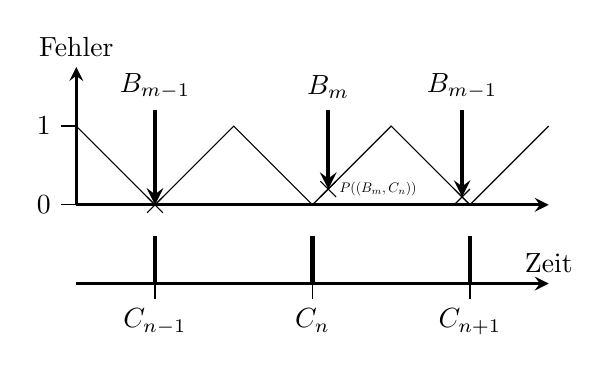
\begin{tikzpicture}
					\tikzstyle{axis} = [very thick, ->, >=stealth]
					\tikzstyle{tick} = [thin];
					\tikzstyle{cbeat} = [ultra thick]
					\tikzstyle{bbeat} = [ultra thick, ->, >=stealth]
					\tikzstyle{graph} = []

					\draw [axis] (0, -1) -- (6, -1) node [anchor=south] {Zeit};
					\draw [axis] (0, 0) -- (6, 0);
					\draw [axis] (0, 0) -- (0, 1.75) node [anchor=south] {Fehler};

					\draw [tick] (0, 0) -- (-0.2, 0) node [anchor=east] {0};
					\draw [tick] (0, 1) -- (-0.2, 1) node [anchor=east] {1};
					\draw [tick] (1, -1) -- (1, -1.2) node [anchor=north] {$C_{n - 1}$};
					\draw [tick] (3, -1) -- (3, -1.2) node [anchor=north] {$C_n$};
					\draw [tick] (5, -1) -- (5, -1.2) node [anchor=north] {$C_{n + 1}$};

					\draw [graph] (0, 1) -- (1, 0) -- (2, 1) -- (3, 0) -- (4, 1) -- (5, 0) -- (6, 1);

					\draw [cbeat] (1, -0.4) -- (1, -1);
					\draw [cbeat] (3, -0.4) -- (3, -1);
					\draw [cbeat] (5, -0.4) -- (5, -1);

					\draw [bbeat] (1, 1.2) node [anchor=south] {$B_{m - 1}$} -- (1, 0);
					\draw [tick] (0.9, -0.1) -- (1.1, 0.1);
					\draw [tick] (0.9, 0.1) -- (1.1, -0.1);
					\draw [bbeat] (3.2, 1.2) node [anchor=south] {$B_m$} -- (3.2, 0.2) node [anchor=west] {\scalebox{0.5}{$P((B_m, C_n))$}};
					\draw [tick] (3.1, 0.1) -- (3.3, 0.3);
					\draw [tick] (3.1, 0.3) -- (3.3, 0.1);
					\draw [bbeat] (4.9, 1.2) node [anchor=south] {$B_{m - 1}$}-- (4.9, 0.1);
					\draw [tick] (4.8, 0.0) -- (5.0, 0.2);
					\draw [tick] (4.8, 0.2) -- (5.0, 0.0);
				\end{tikzpicture}
				\caption{normalisierter Fehler $P$}
			\end{figure}

			% Halb-, Doppeltempo- und Pi-Phase-Fehler
			Beim Erkennen von Beatfolgen,
				treten neben Halbtempo- und Doppeltempofehler auch häufig $\pi$-Phase-Fehler auf.
			Ein $\pi$-Phase-Fehler ist,
				wenn der Beaterkennungsalgorithmus immer genau die Mitte zwischen zwei Beats als Beatvorhersage ausgibt.
			Das tritt häufig bei Liedern auf,
				die zwischen den Hauptschlägen noch Off-Beat-Schläge haben,
				welche lauter oder prägnanter sind als die Hauptschläge.
			Um diese drei Fehlertypen und alle Kombinationen dieser Fehler zu berücksichtigen,
				werden pro Song sechs ``korrekte`` Beatfolgen betrachtet:
				die originale Beatfolge,
				die Halbtempobeatfolge, in der jeder zweite Beat fehlt,
				die Doppeltempobeatfolge, in der zwischen jedem Beat noch ein weiterer Beat eingefügt wird
				und jeweils diese drei Beatfolgen mit einer $\pi$-Phasenverschiebung.

			% Wie alles zusammen kommt
			Eine korrekt vorhergesagte Beatfolge ist eine Folge von Paaren,
				die (1) keine ungepaarten Beats in ihrem Zeitraum hat und
				(2) kein Paar mit einem Fehler von \num{0.35} oder mehr hat.
			Für jeden Algorithmus wird für jedes Lied im Datensatz das oben beschriebene Pairing und die Fehlerberechnung
				sechs Mal berechnet:
				ein Mal für jede der sechs ``korrekten`` Beatfolgen.
			So entstehen sechs Listen von Beatpaaren.
			Die Liste mit der längsten korrekt vorhergesagten Beatfolge,
				wird als die Beatpaarfolge für diesen Song und diesen Algorithmus genommen.
			Die Fehler dieser Beatpaarfolge werden einer Gesamtfehlerliste,
				welche pro Algorithmus existiert und später als Histogram dargestellt wird,
				hinzugefügt.
			Die Fehler der ungepaarten Beats werden ebenfalls dieser Gesamtfehlerliste hinzugefügt.
		}

		\paragraph{Rechenzeit}
		{
			Die relative Rechenzeit eines Algorithmus ergibt sich aus der Division der für alle Lieder benötigten CPU-Zeit durch die gesamte Dauer aller Lieder.
			Diese Zahl gibt an,
				wie viele Sekunden CPU-Zeit ein Algorithmus benötigt um eine Sekunde Audiodaten zu verarbeiten
				und erreicht bei Echtzeitalgorithmen maximal einen Wert von \num{1}.
		}
	}
}

	\chapter{Ergebnisse und Auswertung}
\label{ergebnisse}
\acresetall

% TODO: nochma gucken, was genau in Ergebnisse und was in Auswertung kommt

\section{Tempofehler}
{
	In diesem Abschnitt werden die Daten des Tests dargestellt, ausgewertet und interpretiert,
		die sich auf die Beantwortung der Frage~\ref{question:tempo} beziehen.

	\subsection{Ergebnisse}
	{
		\begin{figure}[h]
			\hspace{-17mm}
			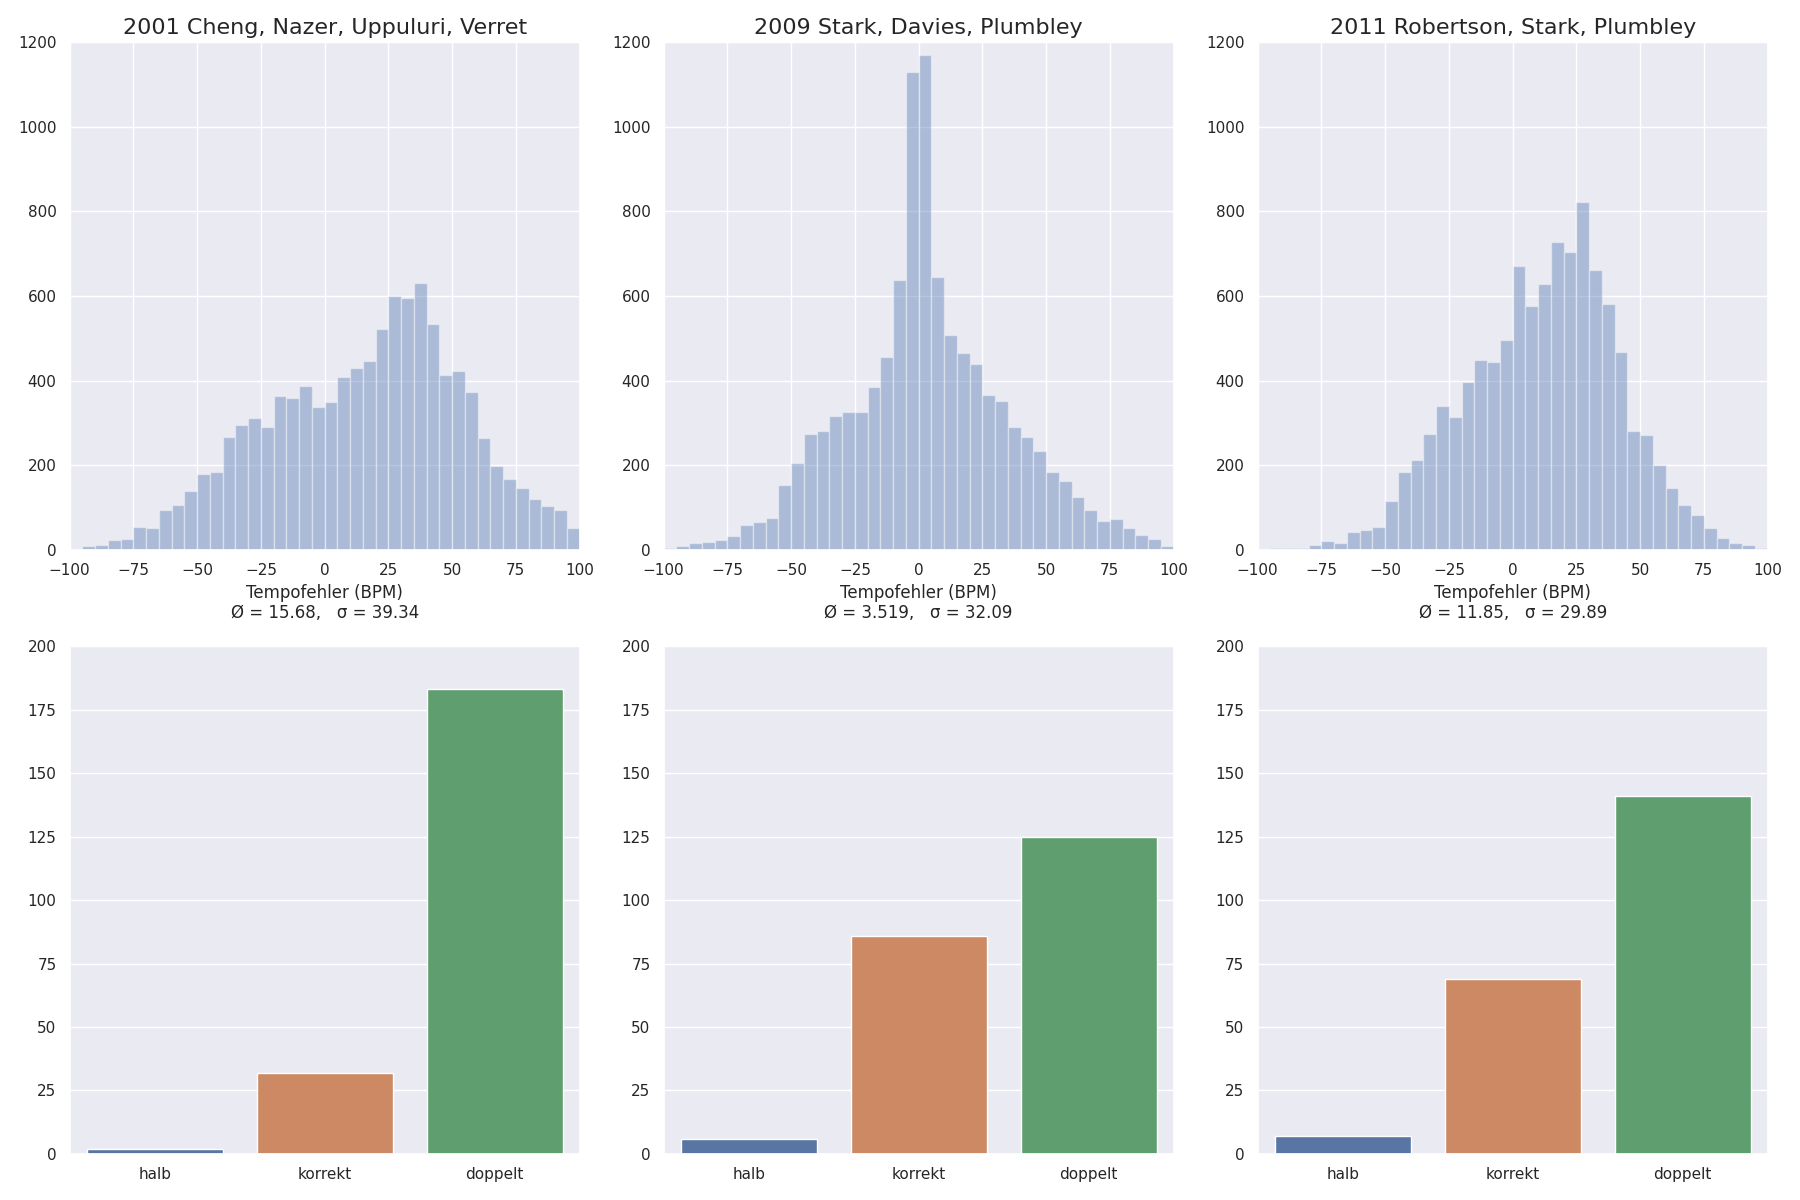
\includegraphics[scale=0.4]{resources/tempo_error_histogram.png}
			\caption{
				oben: Histogramme der Tempofehler, \\
				unten: Anzahl der Lieder, bei denen das halbe/korrekte/doppelte Tempo erkannt wurde
			}
			\label{fig:tempoerror}
		\end{figure}

		% Beschreibung Abbildung Tempofehler
		Die Histogramme in Abbildung~\ref{fig:tempoerror} zeigen die Verteilung der Tempofehler aller Lieder pro Algorithmus.
		Der abgebildete Bereich von \SIrange{-100}{100}{\ac{BPM}} ist in \num{40} Balken unterteilt.
		So umfasst jeder Balken eine Spanne von \SI{5}{\ac{BPM}}.
		Die Balkendiagramme zeigen pro Algorithmus,
			bei wievielen Liedern das halbe, das korrekte oder das doppelte Tempo als Referenztempo genommen wurde.

		% Auffälligkeiten der Abblidung
		Man kann deutlich erkennen,
			dass die Algorithmen von~\cite{2001_BeatThis} und~\cite{2011_PlRoSt} im Durchschnitt das Tempo etwas zu schnell schätzen.
		\cite{2009_DaPlSt} hingegen weicht im Durchschnitt nur minimal von einem Fehler von 0 ab und
			hat mehr Fehler, die sehr nah an 0 sind.
		Am meisten gestreut sind die Fehler bei \cite{2001_BeatThis}.
		Die Fehler von~\cite{2009_DaPlSt} haben zwar eine etwas grö{\ss}ere Streuung (Standardabweichung) als die von~\cite{2011_PlRoSt},
			trotzdem kann man aber sagen,
			dass~\cite{2009_DaPlSt} in diesem Vergleich die besten Tempovorhersagen macht,
			da der Durchschnittsfehler viel näher an 0 ist.

		\begin{figure}[h]
			\centering
			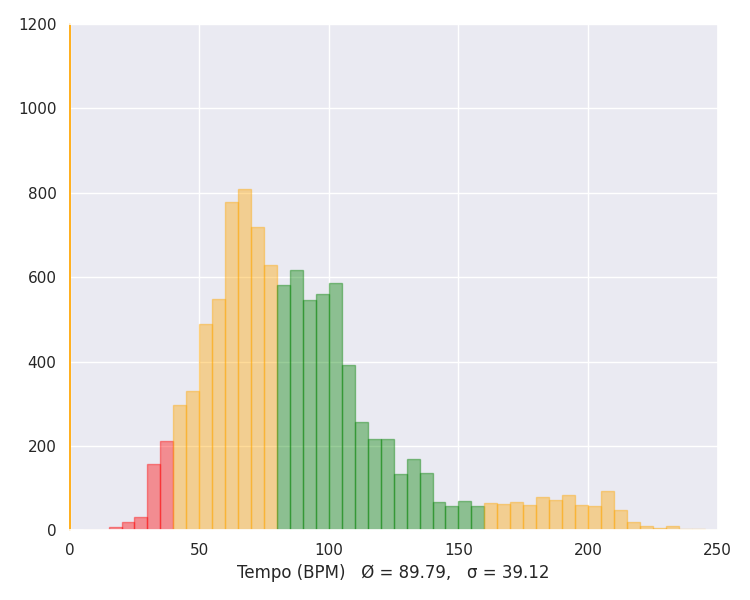
\includegraphics[scale=0.45]{resources/dataset_tempo_histogram.png}
			\caption{Tempoverteilung des Datensatzes}
			\label{fig:dataset_tempo}
		\end{figure}

		Auffällig ist au{\ss}erdem,
			dass bei jedem Algorithmus die meisten Lieder mit dem doppelten Tempo erkannt wurden.
		Das ist hauptsächlich dem limitierten Ausgabebereich der Algorithmen von \SIrange{80}{160}{\ac{BPM}} zu verschulden.
		Abbildung~\ref{fig:dataset_tempo} zeigt die Verteilung der Tempi aller Beatintervalle im Datensatz.
		Der grüne Bereich enthält \SI{44.44}{\percent} aller Beatintervalle
			und markiert den Tempobereich,
			den die Algorithmen direkt ausgeben können (\SIrange{80}{160}{\ac{BPM}}).
		Der gelbe Bereich markiert den Tempobereich,
			den die Algorithmen mit Berücksichtigung von Halb- und Doppeltempofehler ausgeben können,
			also von \SIrange{40}{80}{\ac{BPM}} und von \SIrange{160}{320}{\ac{BPM}},
			und enthält \SI{51.45}{\percent} aller Beatintervalle,
			wobei sich die meisten davon im untern Tempoberiech befinden.
		Das erklärt,
			warum so viele Lieder mit doppeltem Tempo erkannt wurden.
		Der rote Berech ist alles was au{\ss}erhalb von \SIrange{40}{320}{\ac{BPM}} ist
			und markiert den Tempobereich,
			den die Algorithmen unmöglich bestimmen können.
		Dieser Bereich enthält \SI{4.11}{\percent} aller Beatintervalle.
	}

	\subsection{Auswertung}
	{

		% Mögliche Erklärung 1 (ODF)
		Eine mögliche Erklärung,
			warum~\cite{2001_BeatThis} ungenauere Tempovorhersagen macht,
			ist,
			dass der Algorithmus eine einfachere \ac{ODF} verwendet.
		Die \ac{ODF} basiert auf einer Glättung und einer anschliesenden Differentiation.
		So werden nur schnelle Anstiege der Lautstärke extrahiert,
			während bei der \ac{ODF} der anderen beiden Algorithmen auch die Änderungen der Phase im Signal berücksichtigt werden
			und so auch Tonänderungen,
			bei denen die Lautstärke gleich bleibt,
			als Einsätze erkannt werden.

		% Mögliche Erklärung 2 (Tempo Induction)
		Au{\ss}erdem verwendet~\cite{2001_BeatThis} zur Tempobestimmung Kammfilter mit drei Zähnen,
			welche einen ähnlichen Effekt wie eine \ac{ACF} haben.
		Bei der \ac{ACF} wird das Signal mit einer verzögerten Version von sich selbst elementweise multipliziert.
		Bei diesem Kammfilter wird das Signal mit zwei verzögerten Versionen von sich selbst elementweise addiert.
		Beide Operationen haben den Effekt,
			dass sich,
			bei der richtigen Verzögerung,
			die regelmäsigen Peaks des Signals überlagern
			und so die Ausgabe einen gro{\ss}en Wert annimmt.
		Weil ein Signal,
			was sich beispielsweise alle $T$ Sekunden wiederholt,
			sich gleichzeitig auch alle $2T, 3T,$ usw. Sekunden wiederholt,
			entstehen in der \ac{ACF} sowie in der Kammfilterausgabe mehrere Peaks jeweils bei Vielfachen des ersten Peaks.
		\cite{2001_BeatThis} hört an dieser Stelle auf
			und bestimmt einfach den grö{\ss}ten Peak als Beatperiode des Songs,
			während die anderen Peaks ignoriert werden.
		\cite{2009_DaPlSt} hingegen multipliziert anschlie{\ss}end die Ausgabe der \ac{ACF} mit mehreren Kammfiltern
			um die Abstände von äquidistanten Peaks in der \ac{ACF} zu ermitteln.

		% 2009 vs. 2011 (vorverarbeitete ODF)
		Die Tempobestimmung von~\cite{2011_PlRoSt} lässt sich schwierig mit der der anderen beiden Algorithmen vergleichen,
			da sie auf einem komplett anderen Prinzip aufbaut.
		Es lässt sich aber in der Visualisierung der Algorithmen erkennen,
			dass die vorverarbeitete \ac{ODF} von~\cite{2009_DaPlSt} deutlichere und prägnantere Peaks hat,
			als die von~\cite{2011_PlRoSt}.
		Das könnte teilweise die unterschiedlichen Ergebnisse dieser beiden Algorithmen erklären.

		% 2009 vs. 2011 (Einlaufzeit)
		Eine weitere Erklärung für die schlechteren Ergbnisse von~\cite{2011_PlRoSt} könnte eine längere Einlaufzeit sein.
		Vielleicht ist die Tempovorhersage am Ende des Songs nicht ungenauer als die von~\cite{2009_DaPlSt}
			und der Algorithmus braucht nur länger um darauf zu kommen,
			weshalb am Anfang des Songs viele Tempovorhersagen falsch seien könnten
	}
}

\section{Beatzeitpunktfehler}
{
	\label{ergebnisse/beatzeitpunktfehler}

	In diesem Abschnitt werden die Daten des Tests dargestellt, ausgewertet und interpretiert,
		die sich auf die Beantwortung der Frage~\ref{question:beat} beziehen.

	\subsection{Ergebnisse}
	{
		\begin{figure}[h]
			\centering
			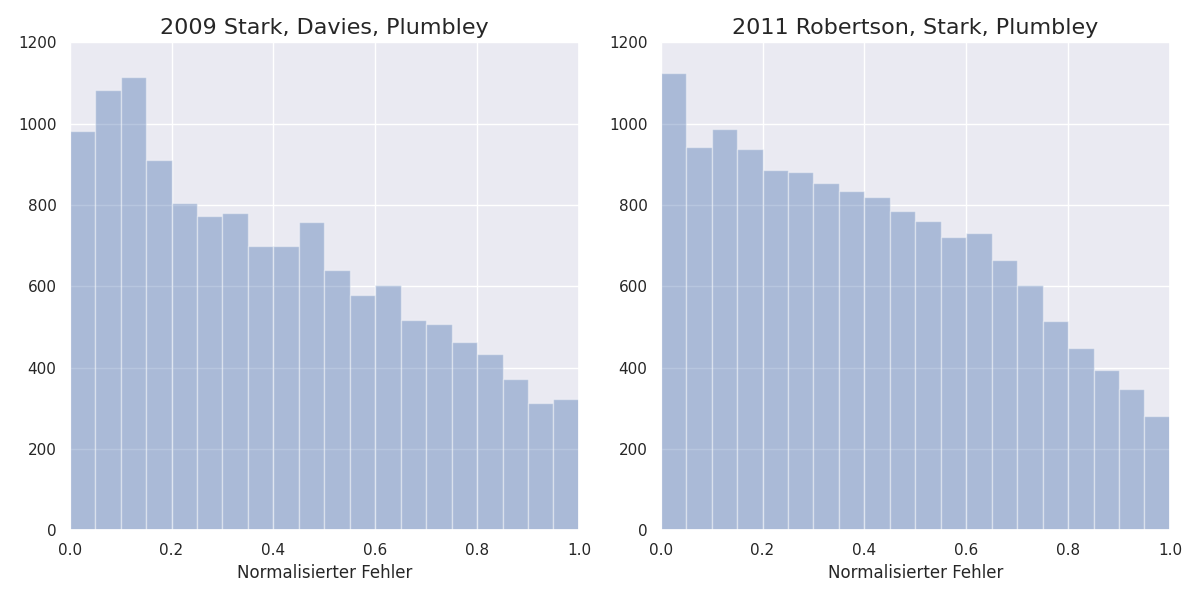
\includegraphics[scale=0.47]{resources/beat_positions.png}
			\caption{Histogramme der Beatzeitpunktfehler}
			\label{fig:beaterror}
		\end{figure}

		\begin{table}[h]
			\centering
			\begin{tabular}{l | r | r}
				                            & \cite{2009_DaPlSt} & \cite{2011_PlRoSt} \\
				\hline \hline
				Anzahl korrekter Beats      & \num{14944}        & \num{15951}        \\
				davon ungepaart             &  \num{1600}        &  \num{1437}        \\
				\hline
				Anzahl vorhergesagter Beats & \num{16361}        & \num{24426}        \\
				davon ungepaart             &  \num{3017}        &  \num{9912}        \\
				\hline
				Anzahl der Beatpaare        & \num{13344}        & \num{14514}
			\end{tabular}
			\caption{Anzahl korrekter und vorhergesagter Beats}
			\label{tab:pairnum}
		\end{table}

		In Abbildung~\ref{fig:beaterror} ist die Verteilung der Fehler aller Beatpaare zu sehen.
		Die Histogramme zeigen nur die Fehler,
			der gepaarten Beats,
			enthalten jedoch keine Informationen über die ungepaarten Beatvorhersagen.
		Wieviele der korrekten und vorhergesagten Beats gepaart wurden,
			kann aus Tabelle~\ref{tab:pairnum} entnommen werden.
		Die unterschiedlichen Zahlen für die Anzahl korrekter Beats kommen daher,
			dass die Lieder,
			je nachdem ob sie der Algorithmus mit halbem, korrektem oder doppeltem Tempo erkennt,
			unterschiedlich viele Beats haben.
	}

	\subsection{Auswertung}
	{
		% Histogramauswertung
		In den beiden Histogrammen kann man erkennen,
			dass beide Algorithmen eine ähnliche Fehlerverteilung haben,
			welche auch zeigt,
			dass es mehr Beatvorhersagen in der Nähe der korrekten Beats gibt.
		Diese Information bezieht sich jedoch nur auf die gepaarten Schläge.
		Aus Tabelle~\ref{tab:pairnum} kann abgelesen werden,
			dass zwar beide Algorithmen ungefär gleich viele Beatvorhersagen hätten machen müssen (Anzahl korrekter Beats),
			aber~\cite{2011_PlRoSt} viel mehr Beatzeitpunkte ausgegeben hat (Anzahl vorhergesagter Beats),
			was zu Folge hatte,
			dass es öfter dazu kam,
			dass mehrere vorhergesagte Beats in die Nähe eines korrekten Beats fielen
			und somit mehr ungepaarte Beats generiert wurden.
		Das hei{\ss}t also,
			dass die Beatvorhersagen von beiden Algorithmen ungefär die gleiche Genauigkeit haben,
			aber~\cite{2011_PlRoSt} zu viele Beats ausgibt.

		% Erklärung
		Eine mögliche Erklärung dafür ist,
			dass \cite{2011_PlRoSt} das Tempo zu schnell schätzt,
			was auch durch Abbildung~\ref{fig:tempoerror} bestätig wird.
		Dadurch werden auch mehr Schläge pro Minute ausgegeben.
		Oft bleibt der Algorithmus auch auf einer Tempo-Phase-Hypothese hängen.
		Wenn diese weit genug weg von den tatsächlichen Werten von Tempo und Phase ist,
			bewirkt die Tempoupdateregel ---
			deren eigentlicher Zweck es ist,
			dass die Tempo-Phase-Hypothese nicht zu schnell zu weit springen kann ---
			dass sich die Ausgabe von Tempo und Phase überhaupt nicht ändert.
	}
}

\section{längste korrekte Beatfolge}
{
	In diesem Abschnitt werden die Daten des Tests dargestellt, ausgewertet und interpretiert,
		die sich auf die Beantwortung der Frage~\ref{question:streak} beziehen.

	\subsection{Ergebnisse}
	{
		\begin{figure}[h]
			\centering
			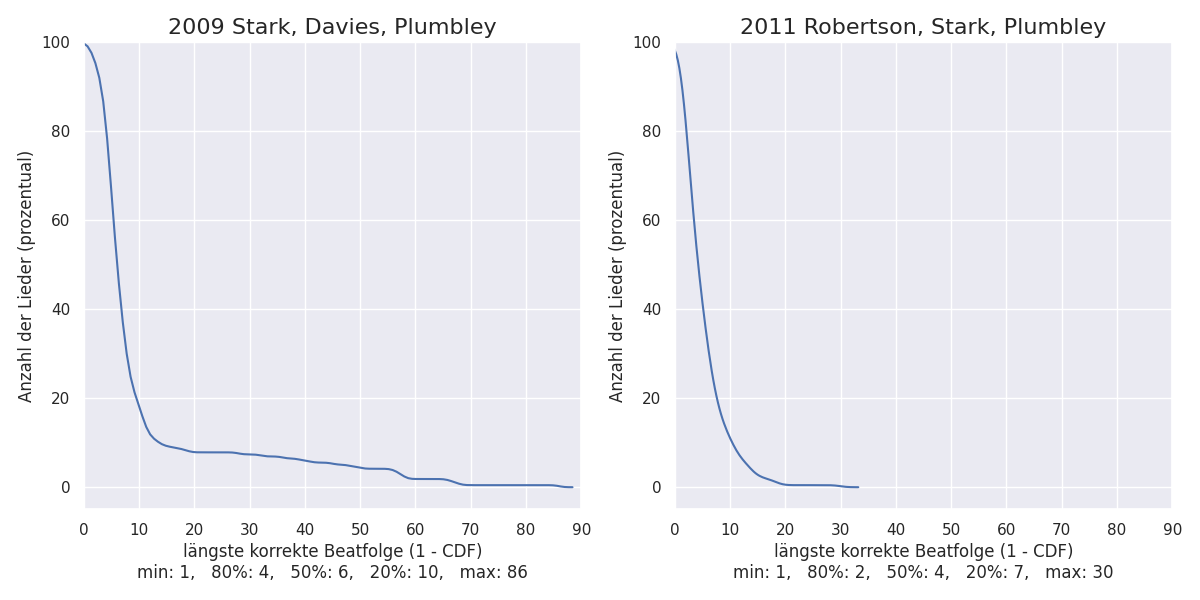
\includegraphics[scale=0.47]{resources/longest_streak.png}
			\caption{Verteilung der längsten korrekten Beatfolgen}
			\label{fig:longest_streak}
		\end{figure}

		Die Graphen in Abbildung~\ref{fig:longest_streak} zeigen eine vertikel gespiegelte kumulative Verteilunsfunktion.
		So kann man für jede Beatfolgenlänge ablsesen,
			in wievielen Liedern (prozentual) eine korrekte Beatfolge mit mindestens dieser Länge erkannt wurde.

		Die längste korrekte Beatfolge von~\cite{2009_DaPlSt} ist \num{86}.
		\cite{2011_PlRoSt} hingegen hat maximal eine  Beatfolge von \num{30} Schlägen korrekt erfasst.
		Generell hat~\cite{2009_DaPlSt} für jede beliebige Beatfolgenlänge eine grö{\ss}ere Anzahl an Liedern,
			bei denen eine mindesten so lange Beatfolge korrekt erfasst wurde.
	}

	\subsection{Auswertung}
	{
		Die Ergebnisse hier lassen sich genauso wie die Ergebnisse in Abschnitt~\ref{ergebnisse/beatzeitpunktfehler} erklären.
		Wahrscheinlich hat~\cite{2011_PlRoSt} das Tempo zu schnell geschätzt,
			wodurch zu viele Beatzeitpunkte ausgegeben wurden.
		Dadurch wird natürlich jede lange korrekte Beatfolge durch viele ungepaarte Beats unterbrochen.
	}

}

\section{Rechenzeit}
{
	In diesem Abschnitt werden die Daten des Tests dargestellt, ausgewertet und interpretiert,
		die sich auf die Beantwortung der Frage~\ref{question:cpu_time} beziehen.

	\subsection{Ergebnisse}
	{
		\begin{table}[h]
			\centering
			\begin{tabular}{l | r | r | r}
				                       & \cite{2001_BeatThis} & \cite{2009_DaPlSt}   & \cite{2011_PlRoSt} \\
				\hline \hline
				Gesamtrechenzeit       & \SI{979.1}{\second}  & \SI{352.2}{\second} & \SI{2796}{\second} \\
				pro Sekunde Audioinput & \SI{112.8}{\milli\second} & \SI{40.58}{\milli\second} & \SI{322.1}{\milli\second}
			\end{tabular}
			\caption{Rechenzeiten der Algorithmen}
			\label{tab:cputime}
		\end{table}

		Tabelle~\ref{tab:cputime} zeigt die Gesamtrechenzeiten,
			die jeder Algorithmus für die Verarbeitung aller Lieder im Datensatz gebraucht hat,
			sowie die benötigte Rechenzeit pro Sekunde Audioeingabe
			also die Zeit,
			die im Durchschnitt benötigt wird um \num{44100} Audiosamples zu verarbeiten.
		Die Gesamtlänge aller Lieder im Datensatz beträgt \num{8680} Sekunden.
	}

	\subsection{Auswertung}
	{
		% Who wins?
		Die Zahlen sind an sich nicht besonders aussagekräftig,
			da sie stark von der verwendeten Hardware abhängen.
		Da aber alle Algorithmen auf der gleichen Hardware getestet wurden,
			lassen sich die Zahlen untereinander vergleichen.
		So geht auch aus diesem Test~\cite{2009_DaPlSt} als klarer Gewinner hervor,
			gefolgt von~\cite{2001_BeatThis} und zuletzt~\cite{2011_PlRoSt}.

		% Erklärung
		Die Unterschiede in der Rechenzeit lassen sich zum Einen auf die unterschiedlichen Aktualsierungsraten der Tempovorhersagen
			und zum Anderen auf die unterschiedlichen Datenmengen,
			die die Algorithmen verarbeiten,
			zurückführen.
		% Updatezeiten
		Während~\cite{2009_DaPlSt} die Tempoberechnung nur alle \num{1.5} Sekunden durchführt,
			aktuallisiert die für diese Arbeit angefertige Implementierung von~\cite{2001_BeatThis} die Tempovorhersage jede Sekunde
			und~\cite{2011_PlRoSt} sogar nach jedem \ac{ODF}-Sample,
			also alle \num{11.61} Millisekunden.
		% Datenmengen
		Au{\ss}erdem arbeitet \cite{2001_BeatThis} direkt auf Audiosamples,
			mit einer Abtastfrequenz von \SI{44.1}{\kilo\hertz},
			statt auf einer \ac{ODF} mit einer Abtastfrequenz von \SI{86}{\hertz} ($1 / \SI{11.61}{\milli\second}$).
		Dadurch ist der \num{1.08} Sekunden lange Anlyserahmen schon $\SI{1.08}{\second} \cdot \SI{44.1}{\kilo\hertz} \cdot \SI{4}{\byte} = \SI{187}{\kibi\byte}$ lang (\num{4} Byte pro Sample, da das Single-Precision-Gleitkommaformat aus dem \acs{IEEE} 754 Standard verwendet wurde).
		Dazu kommt,
			dass~\cite{2001_BeatThis} zwei mal eine \ac{FFT} und eine \ac{IFFT} mit einer Zeitkomplexität von $O(n\log(n))$ auf diesem Array berechnet,
			während~\cite{2009_DaPlSt} fast nur Operationen mit linearer Zeitkomplexität ausführt.
		Die anderen beiden Algorithmen berechnen zwar auch eine \ac{STFT} auf dem Eingangssignal,
			was nichts anderes als eine wiederholte \ac{FFT} ist,
			jedoch nur auf jeweils \num{512} Samples gro{\ss}en Arrays.
		Der Analyserahmen von~\cite{2009_DaPlSt} umfasst zwar \num{6} Sekunden
			ist aber nur \num{512} Samples lang,
			da das \ac{ODF}-Samples sind.
		So werden hier in jedem Verarbeitungsschritt viel kleiner Datenmengen verarbeitet.
		Auch die Kammfiltermatrix aus~\cite{2011_PlRoSt} basiert auf \ac{ODF}-Samples
			und besteht deshalb nur aus $32 + 33 + ... + 65 = 1649$ Samples.
		Diese wird pro Temposchätzung zwei Mal komplett durchlaufen.

		Zusammenfassend kann man also sagen:
		\cite{2011_PlRoSt} verarbeitet wenig Daten,
			jedoch mit einer hohen Aktualisierungsrate,
			wodurch der gro{\ss}e Rechenaufwand zustande kommt.
		\cite{2001_BeatThis} verarbeitet viele Daten,
			jedoch mit einer geringen Aktualisierungsrate,
			wodurch auch ein gro{\ss}er Rechenaufwand zustande kommt.
		\cite{2009_DaPlSt} verarbeitet kleine Datenmengen
			und das auch mit einer geringen Aktualisierungsrate,
			woruch der geringe Rechenaufwand zustande kommt.

		Abschlie{\ss}end muss auch gesagt werden,
			dass die gemessenen Zeiten natürlich implementierungsabhängig sind.
		Das Aktualisierungsinterval von einer Sekunde bei~\cite{2001_BeatThis} ist beispielsweise willkürlich gewählt
			und es gibt in den Implementierungen sicher noch eignige Möglichkeiten für Optimierungen.
		Die ausschlaggebenden Faktoren,
			mit denen die unterschiedlichen Rechenzeiten erklärt wurden,
			also Grö{\ss}e der Analyserahmen,
			Updateinterval des 2009er und 2011er Algorithmus,
			etc.,
			kommen von den Algorithmenbeschreibungen der ursprünglichen Paper
			und sind nicht der Implementierung zu verschulden.
	}
}

	\chapter{Zusammenfassung}
\label{zusammenfassung}

\section{Fazit}
{
	Im Rahmen dieser Arbeit sollte eine Auswahl von Beaterkennungsalgorithmen implementiert
		und mit Hilfe von verschiedenen Tests verglichen werden.
	Es wurden die Algorithmen \cite{2001_BeatThis}, \cite{2009_DaPlSt} und \cite{2011_PlRoSt} ausgewählt und implementiert.
	Vier Tests wurden entworfen und implementiert,
		die die Algorithmen auf Genauigkeit der Tempovorhersage, Genauigkeit der Beatzeitpunkte, längste korrekte Beatfolge und Rechenzeit testen,
		wobei \cite{2001_BeatThis} nur auf Genauigkeit der Tempovorhersage und auf Rechenzeit getestet wurde,
		weil dieser Algorithmus keine Beatzeitpunkte ausgibt.
	Für den Test wurde der Datensatz von~\cite{2012_HoDaZaOlGo} verwendet,
		welcher für Beaterkennungsalgorithmen besonders schwierige Lieder enthält.
	Der Algorithmus von~\cite{2009_DaPlSt} schnitt beim Test auf Genauigkeit der Tempovorhersage am besten ab.
	Die anderen beiden Algorithmen schätzten bei einem Gro{\ss}teil der Lieder das Tempo zu schnell ein.
	Das verursachte bei~\cite{2011_PlRoSt},
		dass der Algorithmus zu viele Beats ausgab,
		weshalb auch die Tests auf Genauigkeit der Beatzeitpunkte und längste korrekte Beatfolge bei \cite{2009_DaPlSt} besser ausfielen.
	Auch beim Test auf Rechenzeit,
		schnitt~\cite{2009_DaPlSt} am besten ab,
		gefolgt von \cite{2001_BeatThis} und \cite{2011_PlRoSt}.
	Die Unterschiede in der Rechenzeit sind hauptsächlich auf die unterschiedlichen Datenmengen,
		die die Algorithmen intern verarbeiten,
		und die unterschiedlichen Aktualisierungsraten der Tempo- und Beatzeitpunktvorhersage zurückzuführen.
}

\section{Ausblick}
{
	% leichteren Datensatz nehmen
	Aufgrund der relativ schlecht ausgefallenen Testergebnisse,
		besteht die Möglichkeit,
		dass in vielen Liedern die Algorithmen gar keinen Takt finden konnten,
		weil der verwendete Datensatz zu schwer war.
	Würde man in zukünftigen Arbeiten die Algorithmen mit einem leichteren Datensatz testen,
		könnte man eventuell feinere Leistungsunterschiede feststellen.

	% mehr Sachen testen
	Die Messung von anderen Metriken kann auch weitere hilfreiche Informationen für die Auswahl eines Beaterkennungsalgorithmus für einen bestimmten Anwendungfall bringen.
	Eine Trennung der Testergebnisse nach Musikrichtung z. B. könnte Aufschlüsse über die Eignung der Algorithmen für bestimmte Genres geben,
		welche wiederum für die Auswahl eines Algorithmus für die Lichtsteuerung eines Live-Auftritts hilfreich sein kann.
	Auch Metriken wie die Einlaufzeit,
		also die Zeit,
		die ein Algorithmus braucht um vom Kaltstart auf das richtige Ergebniss zu kommen,
		oder die Eignung eines Algorithmus für bestimmte Taktarten,
		können hilfreiche Informationen für die Benutzer dieser Algorithmen hervorbringen.

	% krassere Algorithmen testen
	Zukünftige Forschungen könnten au{\ss}erdem weitere state-of-the-art Beaterkennungsalgorithmen vergleichen,
		wie zum Beispiel~\cite{2000_Di} und \cite{2001_Go},
		die für diese Arbeit aufgrund fehlender Informationen nicht implementiert werden konnten,
		oder auch neuere Algorithmen.
	Manche Algorithmen geben speziellere Metainformationen zu den einzelnen Beats aus,
		wie zum Beispiel der Algorithmus von~\cite{2001_Go},
		welcher für jedern Beat bestimmt,
		auf welchem der vier Hauptschläge des 4/4-Takts sich der Beat befindet.
	Solche Algorithmen bieten wiederum eine Grundlage für speziellere Tests.
}


	% Anhang
	\renewcommand{\appendixtocname}{Anhang}
	\renewcommand{\appendixname}{Anhang}
	\renewcommand{\appendixpagename}{Anhang}
	\renewcommand\thesection{\Alph{section}} \renewcommand{\setthesection}{\Alph{section}}
	\setcounter{chapter}{0}

	\cleardoublepage
	\addappheadtotoc
	\let\appendixpagenameorig\appendixpagename
	\renewcommand{\appendixpagename}{\normalfont\sffamily\Huge\mdseries\appendixpagenameorig}
	\appendixpage

	\begin{appendices}
		\begin{subappendices}
			\chaptermark{Literaturverzeichnis}
			\bibliography{references}
			\renewcommand{\listfigurename}{B \hspace{2.25mm} Abbildungsverzeichnis}
			\newpage
			\markboth{Abbildungsverzeichnis}{Abbildungsverzeichnis}
			\listoffigures
			\renewcommand{\listtablename}{C \hspace{2.25mm} Tabellenverzeichnis}
			\newpage
			\listoftables
			\markboth{Tabellenverzeichnis}{Tabellenverzeichnis}
			% GLOSSAR
			\stepcounter{section} \stepcounter{section}
			\newpage
			\section{Abkürzungsverzeichnis}
			\markboth{D \hspace{2.25mm} ABKÜRZUNGSVERZEICHNIS}{D \hspace{2.25mm} ABKÜRZUNGSVERZEICHNIS}
			\begin{acronym}[ODF]
				\acro{ACF}{Autokorrelationsfunktion}
				\acro{API}{Application Programming Interface}
				\acro{BPM}{Beats pro Minute}
				\acro{CD}{Compact Disc}
				\acro{CPU}{Central Processing Unit}
				\acro{CSV}{Comma-Separated Values}
				\acro{FFT}{Schnelle Fourier-Transformation}
				\acro{IEEE}{Institute of Electrical and Electronics Engineers}
				\acro{IFFT}{Inverse Schnelle Fourier-Transformation}
				\acro{ODF}{Einsatzdetektionsfunktion}
				\acroplural{ODF}{Einsatzdetektionsfunktionen}
				\acro{PCM}{Puls-Code-Modulation}
				\acro{STFT}{Kurzzeit-Fourier-Transformation}
			\end{acronym}
		\end{subappendices}
	\end{appendices}
\end{document}
\backmatter
